\documentclass{article}
\usepackage{amsmath}
\usepackage{amssymb}
\usepackage[a4paper, top=25mm, bottom=25mm, left=25mm, right=25mm]{geometry}
\usepackage{pgfplots}
\pgfplotsset{compat=1.18}
\usepackage{mathtools}
\usepgfplotslibrary{polar}
\usepgfplotslibrary{fillbetween}

\begin{document}
\pagestyle{empty}
\large

\begin{center}
2023-2024 Spring \\MAT124 Final\\(04/06/2024)
\end{center}

\noindent 1. Using Lagrange multipliers, find the closest point of the plane $x+z+1=0$ to the point $(1,2,0)$.

\hfill

\noindent 2. Sketch the region and reverse the order of the double integral

\[
\int_0^1
\int_0^{x^2/2}dy\,dx+\int_1^{\sqrt2}\int_{x^2-1}^{x^2/2}dy\,dx\]

\hfill

\noindent 3. Sketch the region and use a double integral in polar coordinates to find the area inside the cardioid $r=1-\cos\theta$ outside the circle $r=1$.

\hfill

\noindent 4. Sketch the region and use a double integral to find the volume of the solid bounded above by the plane $x=z$ and below in the $xy$-plane by the part of the disk $x^2+y^2\leq4$ in the fourth quadrant.

\hfill

\noindent 5. Find the surface area of the portion of the paraboloid $z=25-x^2-y^2$ that lies above the $xy$-plane.

\hfill

\noindent 6. Using the change of variables $u=x-y$ and $v=x+y$, evaluate the integral

\[\iint_{\mathcal{R}}(x-y)\sin\left(x^2-y^2\right)\,dy\,dx\]

\hfill

\noindent where $\mathcal{R}$ is the region bounded by the lines $x+y=1$ and $x+y=3$ and the curves $x^2-y^2=-1$ and $x^2-y^2=1$.

\hfill

\noindent 7. Let $R$ be the solid region bounded by the cone $z=\sqrt{3x^2+3y^2}$ and above by the sphere $x^2+y^2+z^2=9$. Let

\[\mathrm{I}=\iiint_R\left(x^2+y^2\right)\,dV\]

\hfill

\noindent (i) Express (but do not evaluate) $\mathrm{I}$ as a triple integral in spherical coordinates.

\hfill

\noindent (ii) Express (but do not evaluate) $\mathrm{I}$ as a triple integral in cylindrical coordinates.

\newpage

\begin{center}
2023-2024 Spring Final (04/06/2024) Solutions\\
(Last update: 8/4/25 (4th of August) 2:32 PM)
\end{center}

\noindent 1. Let $g(x,y,z)=x+z+1$ and $f(x,y,z)=D^2=(x-1)^2+(y-2)^2+(z-0)^2$. It is easier to work with the square of the distance. Finding the points will not change the result. Solve the system of equations below.

\[
\left.
\begin{array}{l}
\displaystyle\nabla f=\lambda\nabla g \\
\displaystyle g(x,y,z)=0
\end{array}
\right\}\quad
\begin{array}{l}
\nabla f=\left\langle2(x-1),2(y-2),2z\right\rangle=\lambda\left\langle1,0,1\right\rangle=\lambda\nabla g\\\therefore y=2, \quad\lambda=2x-2,\quad\lambda=2z
\end{array}
\]

\begin{equation}2x-2=2z\implies z=x-1\end{equation}

\hfill

\noindent Substitute $(1)$ into the constraint.

\[x+z+1=0\implies x+x-1+1=0\implies2x=0\implies x=0\]
\[\therefore 0+z+1=0\implies z=-1\]

\hfill

\noindent The closest point is then $\boxed{(0,2,-1)}$.

\hfill

\noindent 2.
\begin{center}
\begin{minipage}{0.6\textwidth}
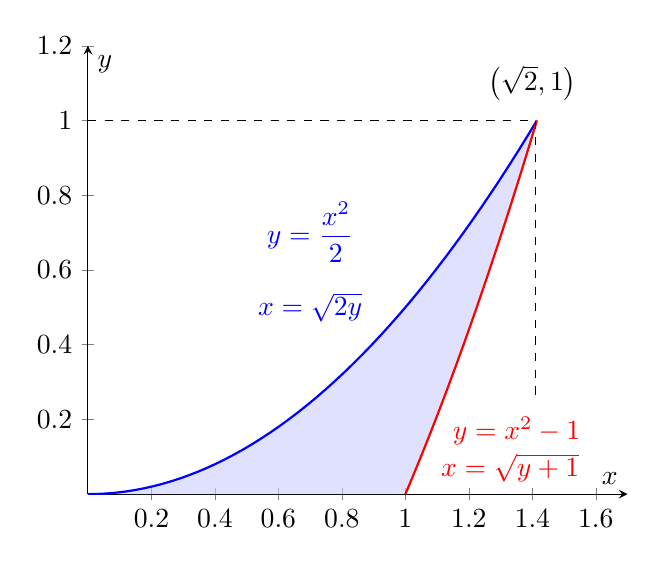
\begin{tikzpicture}
  \begin{axis}[
      axis lines=center,
      xlabel={$x$},
      ylabel={$y$},
      xmin=0, xmax=1.7,
      ymin=0, ymax=1.2,
      samples=50,
      clip=true,
      scale=1,
    ]

    \addplot [
        thick,
        blue,
        domain=0:sqrt(2),
        name path=A,
    ] {x^2/2};

    \addplot [
        thick,
        red,
        domain=1:sqrt(2),
        name path=B,
    ] {x^2-1};
    
    \addplot [
      blue!20,
      fill opacity=0.6,
    ] fill between[of=A and B];

    \node[blue] at (axis cs:0.7,0.7) {$\displaystyle y=\frac{x^2}2$};
    \node[blue] at (axis cs:0.7,0.5) {$x=\sqrt{2y}$};

    \node[red] at (axis cs:1.35,0.17) {$y=x^2-1$};
    \node[red] at (axis cs:1.33,0.07) {$x=\sqrt{y+1}$};
    \node at (axis cs:1.4,1.1) {$\left(\sqrt2,1\right)$};

    \draw[dashed] (0,1) -- (1.41,1);
    \draw[dashed] (1.41,1) -- (1.41,0.25);
  \end{axis}
\end{tikzpicture}
\end{minipage}
\begin{minipage}{0.3\textwidth}
\[\boxed{\int_0^1\int_{\sqrt{2y}}^{\sqrt{y+1}}dx\,dy}\]
\end{minipage}
\end{center}

\hfill

\noindent 3. Find where these two curves intersect and then find the area.

\[1=1-\cos\theta\implies\cos\theta=0\implies\theta=\frac{\pi}2+\pi k,\quad k\in\mathbb{Z}\]

\begin{center}
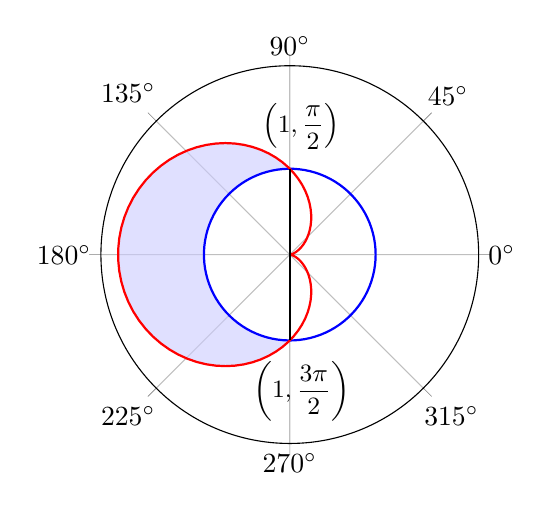
\begin{tikzpicture}
  \begin{polaraxis}[ytick=\empty, axis y line=none, xticklabel=$\pgfmathprintnumber{\tick}^\circ$, samples=100,scale=0.7]
    \addplot [
      domain=pi/2:3*pi/2,
      draw=none,
      name path=A,
      data cs=polarrad,
    ] {1};

    \addplot [
      domain=pi/2:3*pi/2,
      draw=none,
      name path=B,
      data cs=polarrad,
    ] {1-cos(deg(x))};

    \addplot [
      blue!20,
      fill opacity=0.6,
    ] fill between[of=A and B];

    \addplot [
      domain=0:2*pi,
      thick,
      blue,
      data cs=polarrad,
    ] {1};

    \addplot [
      domain=0:2*pi,
      samples=100,
      thick,
      red,
      data cs=polarrad,
    ] {1-cos(deg(x))};

    \draw[black, thick] (axis cs: 90,-1) -- (axis cs: 90,1);
    \node at (axis cs: -85,1.6) {\small$\displaystyle\left(1,\frac{3\pi}2\right)$};
    \node at (axis cs: 85,1.5) {\small$\displaystyle\left(1,\frac\pi2\right)$};

  \end{polaraxis}
\end{tikzpicture}
\end{center}
\begin{align*}
\text{Area}&=\int_{\pi/2}^{3\pi/2}\int_1^{1-\cos\theta}r\,dr\,d\theta=\int_{\pi/2}^{3\pi/2}\left[\frac12r^2\right]_{r=1}^{r=1-\cos\theta}\,d\theta=\frac12\int_{\pi/2}^{3\pi/2}\left[(1-\cos\theta)^2-1^2\right]\,d\theta\\\\&=\frac12\int_{\pi/2}^{3\pi/2}\left(-2\cos\theta+\cos^2\theta\right)\,d\theta=\frac12\int_{\pi/2}^{3\pi/2}\left(-2\cos\theta+\frac{\cos(2\theta)+1}2\right)\,d\theta\\\\&=\frac12\left[-2\sin\theta+\frac{\sin(2\theta)}4+\frac\theta2\right]_{\pi/2}^{3\pi/2}=\frac12\left[\left(2+0+\frac{3\pi}4\right)-\left(-2+0+\frac\pi4\right)\right]=\boxed{2+\frac\pi4}
\end{align*}

\hfill

\noindent 4.

\begin{center}
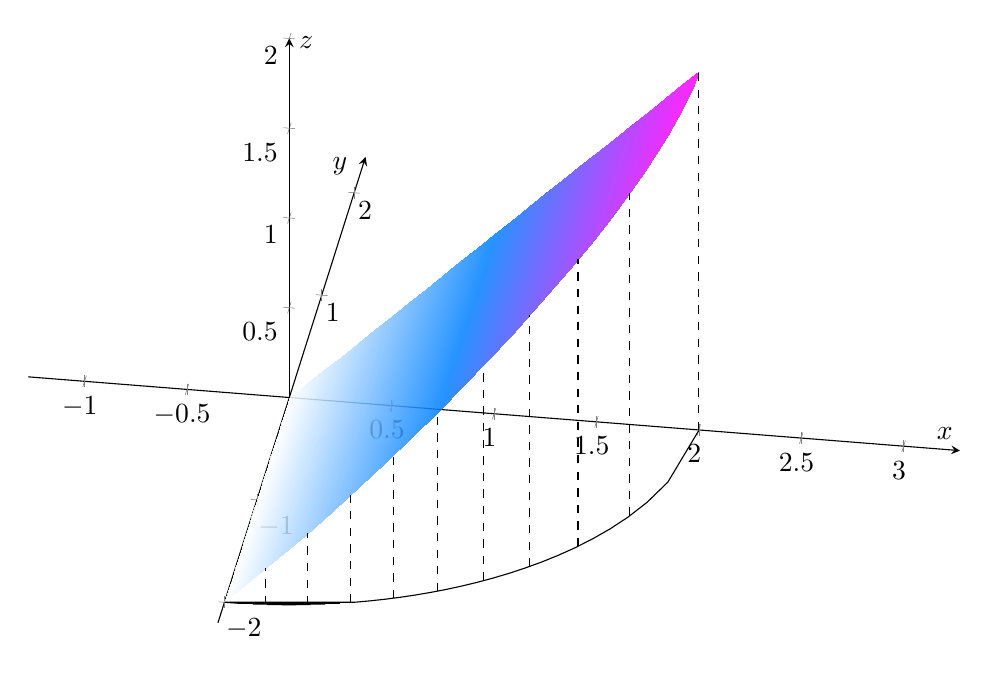
\begin{tikzpicture}
  \begin{axis}[
    view={9}{30},
    axis lines=center,
    xlabel={$x$},
    ylabel={$y$},
    zlabel={$z$},
    domain=0:2,
    ymin=-2.2,
    z buffer=sort,
    colormap/cool,
    axis equal,
    scale=2,
    ]
    
    \addplot3[surf, shader=interp, opacity=0.85, y domain=270:360] ({x * cos(y)}, {x * sin(y)}, {x * cos(y)});
    \addplot3[black, samples=30] ({x}, {-sqrt(4 - x^2)}, {0});
    
    \draw[dashed] (2,0,0)--(2,0,2); \draw[dashed] (1.8,-0.87,0)--(1.8,-0.87,1.8); \draw[dashed] (1.6,-1.2,0)--(1.6,-1.2,1.6); \draw[dashed] (1.4,-1.428,0)--(1.4,-1.428,1.4); \draw[dashed] (1.2,-1.6,0)--(1.2,-1.6,1.2); \draw[dashed] (1,-1.732,0)--(1,-1.732,1); \draw[dashed] (0.8,-1.833,0)--(0.8,-1.833,0.8); \draw[dashed] (0.6,-1.907,0)--(0.6,-1.907,0.6); \draw[dashed] (0.4,-1.959,0)--(0.4,-1.959,0.4); \draw[dashed] (0.2,-1.989,0)--(0.2,-1.989,0.2);
    \end{axis}
\end{tikzpicture}
\end{center}
\[
\begin{array}{c}
x=r\cos\theta\\
y=r\sin\theta\\
x^2+y^2=r^2\\
dA=r\,dr\,d\theta
\end{array}\quad\rightarrow\quad
\begin{array}{c}
z=x\implies z_{\text{upper}}=r\cos\theta\\
z=0\implies z_{\text{lower}}=0\\[0.2cm]
\displaystyle0\leq\theta\leq\frac\pi2
\end{array} 
\]

\hfill

\noindent The volume of this solid can be evaluated with the following integral.

\begin{align*}\text{Volume}&=\int_0^{\pi/2}\int_0^2\left(r\cos\theta-0\right)\,r\,dr\,d\theta=\int_0^{\pi/2}\int_0^2r^2\cos\theta\,dr\,d\theta=\int_0^{\pi/2}\left[\frac{r^3}3\right]_{r=0}^{r=2}\cos\theta\,d\theta\\\\&=\frac83\int_0^{\pi/2}\cos\theta\,d\theta=\frac83\sin\theta\,\bigg|_{0}^{\pi/2}=\frac83(1-0)=\boxed{\frac83}
\end{align*}

\newpage

\noindent 5. For $z=0$, we get the circle $x^2+y^2=25$. Therefore, the domain is $x^2+y^2\leq25$. Using the double integral below, we find the surface area.

\begin{align*}
\text{Surface area}&=\iint_D\sqrt{1+\left(\frac{\partial z}{\partial x}\right)^2 +\left(\frac{\partial z}{\partial y}\right)^2}\,dA\\\\&=\int_{-5}^5\int_{-\sqrt{25-x^2}}^{\sqrt{25-x^2}}\sqrt{1+\left(-2x\right)^2 +\left(-2y\right)^2}\,dy\,dx\\\\&=\int_{-5}^5\int_{-\sqrt{25-x^2}}^{\sqrt{25-x^2}}\sqrt{1+4x^2+4y^2}\,dy\,dx
\end{align*}

\hfill

\noindent If we switch to polar coordinates, we can easily evaluate the integral.

\begin{align*}\text{Surface area}&=\int_0^{2\pi}\int_0^5\sqrt{1+4r^2}\,r\,dr\,d\theta=\int_0^{2\pi}\left[\frac1{12}\left(1+4r^2\right)^{3/2}\right]_{r=0}^{r=5}\,d\theta\\\\&=\frac1{12}\int_0^{2\pi}\left[\left(1+4\cdot25\right)^{3/2}-\left(1+4\cdot0\right)^{3/2}\right]\,d\theta=\frac{101^{3/2}-1}{12}\int_0^{2\pi}d\theta\\\\&=\boxed{\frac{101^{3/2}-1}6\cdot\pi}\end{align*}

\hfill

\noindent 6. Rewrite $x$ and $y$ in terms of $u$ and $v$ and sketch the regions in both coordinates.

\[
\left.
\begin{array}{c}
u=x-y\\v=x+y
\end{array}\right\}
\quad \displaystyle x=\frac{u+v}2,\quad y=\frac{v-u}2
\]

\[x+y=3\implies\frac{u+v}2+\frac{v-u}2=3\implies v=3\]

\[x+y=3\implies\frac{u+v}2+\frac{v-u}2=1\implies v=1\]

\begin{align*}x^2-y^2=1&\implies\left(\frac{u+v}2\right)^2-\left(\frac{v-u}2\right)^2=\frac14\left(u^2+2uv+v^2-v^2+2uv-u^2\right)=1\\\\&\implies u=\frac1v\end{align*}

\begin{align*}y^2-x^2=1&\implies\left(\frac{v-u}2\right)^2-\left(\frac{u+v}2\right)^2=\frac14\left(v^2-2uv+u^2-u^2-2uv-v^2\right)=1\\\\&\implies u=-\frac1v\end{align*}

\begin{center}
\begin{minipage}{0.45\textwidth}
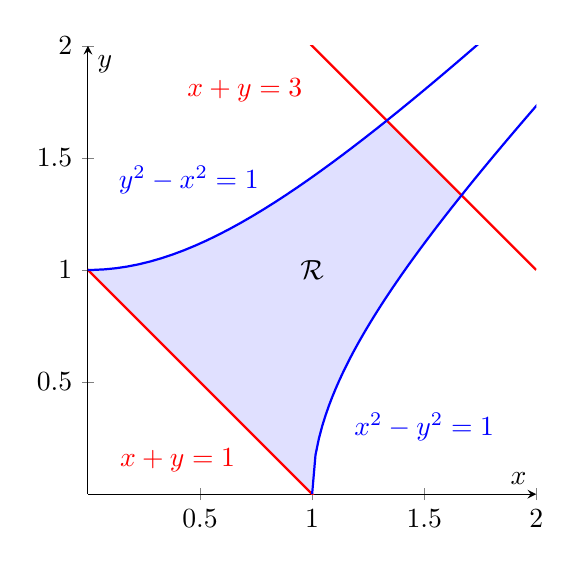
\begin{tikzpicture}
  \begin{axis}[
      axis equal image,
      xmin=0, xmax=2,
      ymin=0, ymax=2,
      axis lines=middle,
      xlabel={$x$}, ylabel={$y$},
      clip=true,
      samples=100,
      scale=1,
    ]

    \addplot[name path=line1, red, thick, domain=-2:2] ({x}, {1 - x});
    \addplot[name path=line2, red, thick, domain=-2:2] ({x}, {3 - x});

    \addplot[name path=hyper1a, blue, thick, domain=-2.5:-1.1] ({x}, {sqrt(x^2 - 1)});
    \addplot[name path=hyper1b, blue, thick, domain=1:2.5] ({x}, {sqrt(x^2 - 1)});
    \addplot[name path=hyper2a, blue, thick, domain=-2.5:2.5] ({x}, {sqrt(x^2 + 1)});

    \addplot [name path=upper, domain=0:5/3, draw=none] ({x}, {min(3 - x, sqrt(1+x^2))});

    \addplot [name path=lower, domain=0:5/3, draw=none] ({x}, {max(1 - x, sqrt(x^2 - 1))});

    \addplot [ blue!20, opacity=0.6] fill between [of=upper and lower, soft clip={domain=0:5/3}];

    \node at (axis cs:0.45,1.4) [blue] {$y^2-x^2 = 1$};
    \node at (axis cs:1.5,0.3) [blue] {$x^2 - y^2 = 1$};
    \node at (axis cs:0.4,0.15) [red] {$x + y = 1$};
    \node at (axis cs:0.7,1.8) [red] {$x + y = 3$};
    \node at (axis cs:1,1) {$\mathcal{R}$};
  \end{axis}
\end{tikzpicture}
\end{minipage}$\rightarrow$\begin{minipage}{0.45\textwidth}
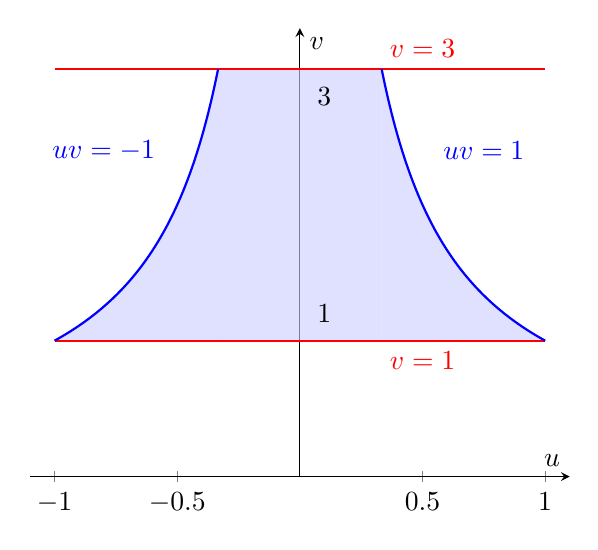
\begin{tikzpicture}
  \begin{axis}[
      xmin=-1.1, xmax=1.1,
      ymin=0, ymax=3.3,
      axis lines=middle,
      xlabel={$u$}, ylabel={$v$},
      clip=true,
      samples=100,
      ytick=\empty,
      scale=1,
    ]

    \addplot[red, thick, domain=-1:1] {3};
    \addplot[red, thick, domain=-1:1] {1};

    \addplot[blue, thick, domain=1/3:1] {(1/x)};
    \addplot[blue, thick, domain=-1:-1/3] {(-1/x)};

    \addplot [name path=upper1,domain=-1:-1/3,draw=none] {-1/x};
    \addplot [name path=upper2,domain=-1/3:1/3,draw=none] {3};
    \addplot [name path=upper3,domain=1/3:1,draw=none] {1/x};

    \addplot [name path=lower, domain=-1:1, draw=none] {1};

    \addplot [blue!20, opacity=0.6] fill between [of=upper1 and lower, soft clip={domain=-1:-1/3}];
    \addplot [blue!20, opacity=0.6] fill between [of=upper2 and lower, soft clip={domain=-1/3:1/3}];
    \addplot [blue!20, opacity=0.6] fill between [of=upper3 and lower, soft clip={domain=1/3:1}];

    \node at (axis cs:-0.8,2.4) [blue] {$uv=-1$};
    \node at (axis cs:0.75,2.4) [blue] {$uv=1$};
    \node at (axis cs:0.5,0.85) [red] {$v=1$};
    \node at (axis cs:0.5,3.15) [red] {$v=3$};
    
    \node at (axis cs:0.1,2.8) {$3$};
    \node at (axis cs:0.1,1.2) {$1$};
  \end{axis}
\end{tikzpicture}
\end{minipage}
\end{center}

\hfill

\noindent Calculate the Jacobian determinant to find the area in terms of $u$ and $v$.

\[
\left|\frac{\partial(x,y)}{\partial(u,v)}\right|=\left|\begin{array}{cc}
\displaystyle\frac{\partial x}{\partial u}&\displaystyle\frac{\partial x}{\partial v}\\[1em]
\displaystyle\frac{\partial y}{\partial u}&\displaystyle\frac{\partial y}{\partial v}
\end{array}\right|=\left|\begin{array}{cc}
\displaystyle\frac12&\displaystyle\frac12\\[1em]
\displaystyle\frac{-1}2&\displaystyle\frac12
\end{array}\right|=\frac12\cdot\frac12-\left(-\frac12\cdot\frac12\right)=\frac12
\]

\hfill

\noindent The integral then becomes

\begin{align*}
\mathrm{I}&=\iint_{\mathcal{R}}(x-y)\sin\left(x^2-y^2\right)\,dy\,dx=\int_1^3\int_{-1/v}^{1/v}u\cdot\sin(uv)\cdot\left|\frac{\partial(x,y)}{\partial(u,v)}\right|\,du\,dv\\\\&=\int_1^3\int_{-1/v}^{1/v}u\cdot\sin(uv)\cdot\frac12\,du\,dv
\end{align*}

\hfill

\noindent Multiply each side by $2$ to obviate the mess with the fraction $\displaystyle\frac12$ and then change the order of integration.

\begin{align*}
2\mathrm{I}&=\int_{-1}^{\textstyle-\frac13}\int_1^{\textstyle-\frac1u}u\sin(uv)\,dv\,du+\int_{\textstyle-\frac13}^{\textstyle\frac13}\int_1^3u\sin(uv)\,dv\,du+\int_{\textstyle\frac13}^1\int_1^{\textstyle\frac1u}u\sin(uv)\,dv\,du\\\\&=\int_{-1}^{\textstyle-\frac13}(-\cos(uv))\,\bigg|_{v=1}^{v=-\frac1u}\,du+\int_{\textstyle-\frac13}^{\textstyle\frac13}(-\cos(uv))\,\bigg|_{v=1}^{v=3}\,du+\int_{\textstyle\frac13}^1(-\cos(uv))\,\bigg|_{v=1}^{v=\frac1u}\,du\\\\&=\int_{-1}^{\textstyle-\frac13}[-\cos(-1)+\cos u]\,du+\int_{\textstyle-\frac13}^{\textstyle\frac13}[-\cos(3u)+\cos u]\,du+\int_{\textstyle\frac13}^1[-\cos1+\cos u]\,du\\\\&=\bigg[-u\cos(-1)+\sin u\bigg]_{-1}^{\textstyle-\frac13}+\bigg[-\frac13\sin(3u)+\sin u\bigg]_{\textstyle-\frac13}^{\textstyle\frac13}+\bigg[-u\cos1+\sin u\bigg]_{\textstyle\frac13}^1
\end{align*}

\begin{align*}
2\mathrm{I}&=\left[-\frac23\cos(-1)+\sin\left(-\frac13\right)-\sin(-1)\right]+\left[-\frac13\left(\sin1-\sin(-1)\right)+\sin\frac13-\sin\left(-\frac13\right)\right]\\\\&\quad\:+\left[-\frac23\cos1+\sin1-\sin\frac13\right]\\\\&=\frac43(\sin1-\cos1)
\end{align*}

\noindent This is the value of $2\mathrm{I}$. Therefore, $\boxed{\mathrm{I}=\frac23(\sin1-\cos1)}$.

\hfill

\noindent 7.

\hfill

\noindent (i) For spherical coordinates, we have

\[
\begin{array}{c}
z=\rho\cos\theta\\
r=\rho\sin\theta\\
x^2+y^2=r^2\\
x^2+y^2+z^2=\rho^2\\
dV=\rho^2\sin\phi\,d\rho\,d\phi\,d\theta
\end{array}\quad\rightarrow\quad
\begin{array}{c}
\displaystyle z=\sqrt{3x^2+3y^2}\implies\rho\cos\theta=\sqrt3\rho\sin\theta\implies\theta=\frac\pi6\\[0.2cm]
x^2+y^2=r^2=\rho^2\sin^2\theta\\[0.1cm]
x^2+y^2+z^2=9\implies\rho^2=9\implies\rho=3\\[0.1cm]
0\leq\theta\leq2\pi
\end{array}
\]

\hfill

\noindent The integral in spherical coordinates can be expressed as follows.

\[\boxed{\mathrm{I}=\int_0^{2\pi}\int_0^{\pi/6}\int_{0}^3\rho^2\sin^2\phi\cdot\rho^2\sin\phi\,d\rho\,d\phi\,d\theta=\int_0^{2\pi}\int_0^{\pi/6}\int_{0}^3\rho^4\sin^3\phi\,d\rho\,d\phi\,d\theta}\]

\hfill

\noindent (ii) For cylindrical coordinates, we have

\[
\begin{array}{c}
z=z\\
r^2=x^2+y^2\\
dV=r\,dz\,dr\,d\theta
\end{array}\quad\rightarrow\quad
\begin{array}{c}
z=\sqrt{3x^2+3y^2}\implies z=r\sqrt3\\[0.1cm]
x^2+y^2=r^2\\[0.1cm]
x^2+y^2+z^2=9\implies z=\sqrt{9-r^2}\\[0.1cm]
0\leq\theta\leq2\pi
\end{array}
\]

\hfill

\noindent Find where the curves intersect to find the upper limit of $r$.

\[r\sqrt3=\sqrt{9-r^2}\implies3r^2=9-r^2\implies r^2=\frac94\implies r=\frac32\]

\hfill

\noindent The integral in cylindrical coordinates can be expressed as follows.

\[\boxed{\mathrm{I}=\int_0^{2\pi}\int_0^{3/2}\int_{r\sqrt3}^{\sqrt{9-r^2}}r^2\cdot r\,dz\,dr\,d\theta=\int_0^{2\pi}\int_0^{3/2}\int_{r\sqrt3}^{\sqrt{9-r^2}}r^3\,dz\,dr\,d\theta}\]

\end{document}